% !TeX root = Documentation.tex

\documentclass[12pt,a4paper,english]{report} 

\usepackage[utf8]{inputenc}
\usepackage[provide=*]{babel}
\usepackage{microtype}
\usepackage{graphicx}

\title{Smart Turntable Assistant}
\author{Daniel Kiss}
\date{\today}

\clubpenalty=100000
\widowpenalty=100000

\begin{document}

\maketitle
\tableofcontents

\chapter{Introduction}

In recent years, the music industry has witnessed an unprecedented resurgence in the popularity of analog physical media, specifically vinyl records. Audiophiles and casual listeners alike are drawn to the tactile experience, the deliberate act of listening to an album from start to finish, and the distinct, warm acoustic characteristics of analog sound. However, in an era dominated by digital streaming platforms like Spotify and Apple Music, the traditional vinyl listening experience remains fundamentally disconnected from the modern digital ecosystem. 

This dissertation presents the design, architecture, and implementation of a ``Smart Turntable Assistant''---a software-driven bridge between analog audio hardware and modern digital conveniences. By utilizing real-time audio processing and third-party API integrations, this project aims to modernize the analog listening experience without compromising the physical medium itself.

\section{Problem Statement}

The core limitation of analog audio is that it is a continuous, raw electrical signal entirely devoid of metadata. Unlike digital audio files, a turntable cannot natively inform the listener or surrounding devices about what is currently playing. This technological gap results in several distinct problems for the modern vinyl listener:

\begin{enumerate}
    \item \textbf{Lack of Digital Integration:} Users cannot automatically track their listening habits. Logging plays (scrobbling) to social music platforms like Last.fm requires tedious manual data entry.
    \item \textbf{Absence of Contextual Media:} Modern streaming conveniences, such as synchronized lyrics and high-resolution album artwork displays, are completely unavailable during analog playback.
    \item \textbf{Hardware Degradation Blindness:} Turntable styluses have a limited lifespan, after which they can permanently damage the vinyl grooves. Users currently rely on rough estimations to track cartridge wear.
    \item \textbf{Lack of Accessible Diagnostics:} Identifying issues like excessive motor vibration, surface damage, or inner-groove tracking distortion traditionally requires expensive, dedicated acoustic measurement hardware.
\end{enumerate}

\section{Objectives of the Thesis}

The primary objective of this thesis is to engineer a robust, real-time Client-Server application that passively monitors the audio output of a standard turntable and provides a comprehensive suite of ``smart'' features. The system is designed to run on lightweight hardware connected to a USB Audio Interface.

To solve the problems outlined above, the project defines the following technical objectives:

\begin{itemize}
    \item \textbf{Real-Time Signal Processing:} Develop a concurrent Python backend capable of continuously analyzing the analog audio stream to detect when a song starts or stops, and to mathematically calculate hardware diagnostics.
    \item \textbf{Audio Fingerprinting and Metadata Enrichment:} Implement a robust recognition pipeline that records short audio samples and identifies them using audio fingerprinting services. Furthermore, design a ``waterfall'' metadata retrieval system to reliably fetch exact track durations, album names, and high-resolution artwork.
    \item \textbf{Automated Digital Synchronization:} Create background services to fetch timestamped lyrics and implement automated Last.fm scrobbling that accurately respects the track's elapsed playback time.
    \item \textbf{Database and Hardware Management:} Implement a relational database to persist listening history, save customized vinyl aesthetic preferences, and precisely track the lifecycle of multiple user-defined turntable cartridges.
    \item \textbf{Modern, Reactive User Interface:} Design a responsive Single Page Application using Vue.js that communicates with the backend via WebSockets. The interface must provide users with zero-latency visual feedback and offer dynamic thematic customization.
\end{itemize}

\chapter{Technological Background and Literature Review}

Developing a real-time hardware monitoring and music recognition system requires the integration of multiple disciplines, ranging from digital signal processing to modern web application architecture. This chapter reviews the fundamental technologies, algorithms, and frameworks chosen to implement the Smart Turntable Assistant.

\section{Audio Fingerprinting Technologies}
Objective
Audio fingerprinting is a mechanism used to identify an audio sample by extracting unique acoustic characteristics and comparing them against a known database. Unlike basic metadata tagging, fingerprinting analyzes the actual audio content. The process typically involves converting the audio signal into a spectrogram, identifying points of high energy or peaks, and generating a constellation map. These peaks are then hashed into compact digital signatures.

This mathematical approach is highly resilient to background noise, pitch distortion, and the inherent surface crackle of vinyl records. In this project, industry-standard recognition engines including the Shazam API and ACRCloud are utilized to perform the fingerprint matching. These services compare the recorded audio buffers against massive commercial databases to accurately identify the playing track regardless of analog imperfections.

\section{Applied Frameworks}

The architecture of the application relies on a strict separation of concerns, divided into a robust backend and a dynamic frontend. 

For the backend, Python was selected due to its extensive ecosystem for mathematical computing and digital signal processing. Libraries such as NumPy and SciPy are heavily utilized to perform array manipulations, filter frequencies, and calculate acoustic metrics in real time. The web server layer is powered by Flask. As a lightweight microframework, Flask provides the necessary tools to expose a RESTful API and manage database sessions through the SQLAlchemy object-relational mapper without introducing unnecessary overhead.

The frontend is implemented as a Single Page Application using Vue.js. Vue was chosen for its reactive component-based architecture, which allows the user interface to update instantly as underlying data changes. Global state management is handled by Pinia, ensuring that hardware settings, user authentication status, and current playback metadata remain perfectly synchronized across all application views.

\begin{figure}[htbp]
    \centering
    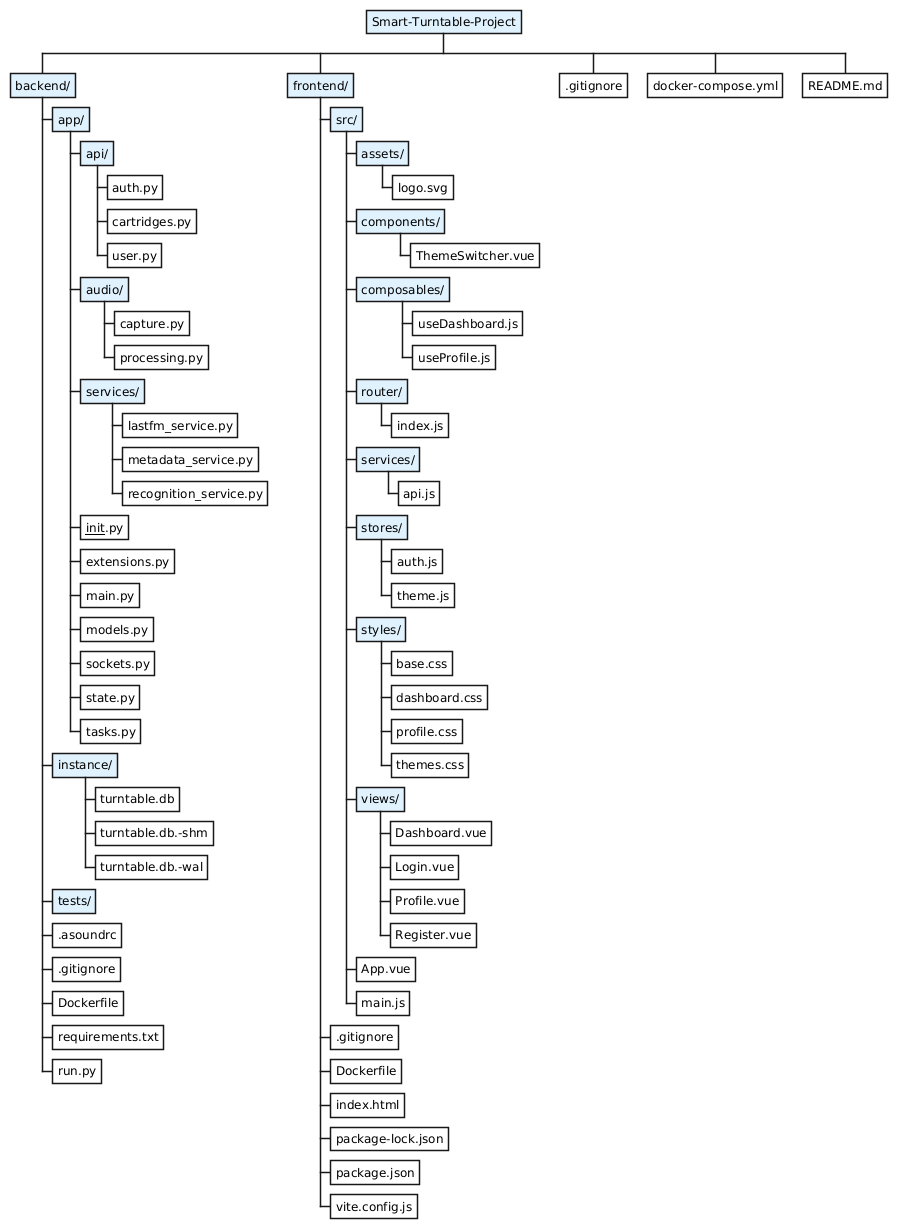
\includegraphics[width=0.9\textwidth]{Images/folder.png}
    \caption{Hierarchical overview of the project's decoupled directory structure.}
    \label{fig:folders}
\end{figure}

\section{Real-Time Communication}

A core requirement of the system is the ability to display hardware diagnostics and synchronized lyrics with zero perceptible latency. Traditional HTTP polling, where the client repeatedly requests data from the server, introduces significant network overhead and is entirely unsuitable for high-frequency audio visualization.

To solve this, the application employs WebSockets. WebSockets establish a persistent, full-duplex communication channel over a single TCP connection. This allows the Python backend to push data outward continuously without waiting for a client request. The Socket.IO library is used to bridge the Flask backend and the Vue frontend, facilitating the seamless broadcasting of volume levels, click detection events, and playback timers at a rate of ten frames per second.

\section{Development and Execution Environment}

Ensuring that the software can run reliably across different operating systems requires strict environment isolation. Docker is utilized for containerization, packaging the entire application along with its system-level dependencies into standardized units. 

A significant challenge in containerizing audio applications is granting the isolated environment access to physical host hardware. This is resolved by mapping the host machine's sound devices into the Docker container, bridging the Advanced Linux Sound Architecture and PulseAudio subsystems. This setup allows the application to be deployed effortlessly on standard desktop computers during development, while remaining perfectly optimized for its final production environment on low-power, single-board computers like the Raspberry Pi.

\chapter{Requirements Analysis}

Before the architectural design and software implementation phases, a comprehensive analysis of the system requirements is necessary. This ensures that the final product successfully bridges the gap between analog audio playback and modern digital conveniences. This chapter outlines the specific functional capabilities the system must possess, the non-functional quality attributes it must adhere to, and the primary use cases defining user interaction.

\section{Functional Requirements}

Functional requirements define the exact behaviors, processes, and features the Smart Turntable Assistant must execute to deliver value to the end user.

\begin{itemize}
    \item \textbf{Real-Time Audio Identification:} The system must continuously monitor the audio input stream and automatically detect when playback begins. Upon detection, it must capture a short audio buffer and query external audio fingerprinting application programming interfaces to identify the track.
    \item \textbf{Metadata Enrichment:} Following a successful audio match, the application must query secondary music databases. This step is required to retrieve high-resolution album artwork, the exact track duration in milliseconds, and the standardized album name.
    \item \textbf{Synchronized Lyrics Display:} The backend must fetch timestamped lyric files for the identified song. The frontend must parse these timestamps and automatically scroll the text in synchronization with the live playback timer. The user must also have the ability to manually offset the synchronization timeline to correct minor mechanical delays.
    \item \textbf{Hardware Condition Diagnostics:} The software must analyze the incoming analog signal to calculate the root mean square volume level. It must mathematically process the audio to detect sudden surface clicks, measure low-frequency mechanical motor rumble, and quantify high-frequency sibilant distortion.
    \item \textbf{Cartridge Lifecycle Management:} The system must maintain a database of user-owned turntable styluses. It must track the cumulative playback time for the currently active hardware, allow the user to define a maximum recommended lifespan, and provide an option to reset the counter when the hardware is replaced.
    \item \textbf{Digital Listening Logs:} The application must support authentication with external social music tracking services like Last.fm. It must automatically log a track to the user profile once a specific playback duration threshold is reached.
    \item \textbf{Aesthetic Customization:} The web interface must allow users to customize the visual representation of the digital record to match colored physical media. This color preference must be saved to the database and automatically reapplied whenever a track from that specific album is played again.
\end{itemize}

\section{Non-Functional Requirements}

Non-functional requirements dictate the performance standards, reliability constraints, and usability metrics that the system architecture must satisfy.

\begin{itemize}
    \item \textbf{Performance and Latency:} The background audio processing thread must operate continuously without blocking the web server operations. Diagnostic data must be broadcast to the frontend multiple times per second to guarantee fluid visual animations and accurate light-emitting diode meter representations.
    \item \textbf{Reliability and Fallback Mechanisms:} Network queries to external databases must implement robust fallback strategies. If a primary recognition engine or metadata service fails, the system must seamlessly attempt secondary sources to prevent missing data and ensure uninterrupted operation.
    \item \textbf{Usability and Responsiveness:} The graphical user interface must scale dynamically across various display sizes, ranging from mobile phone screens to high-resolution desktop monitors. Container queries and fluid typography must be utilized to maintain layout integrity.
    \item \textbf{Database Concurrency:} The underlying relational database must support simultaneous read and write operations. Background threads must be able to update cartridge statistics while the identification thread concurrently saves new track history logs, requiring write-ahead logging to prevent database locking errors.
\end{itemize}

\section{Use Cases}

The following use cases illustrate the primary interactions between the listener and the Smart Turntable Assistant during a typical listening session.

\begin{itemize}
    \item \textbf{Automated Playback Monitoring:} A user drops the needle onto a vinyl record. The system detects the audio threshold, identifies the track, and populates the dashboard with the correct album art and synchronized lyrics without any manual input.
    \item \textbf{Hardware Diagnostic Observation:} A user navigates to the diagnostics tab while a record is playing. They monitor the live interface to verify that the turntable motor is isolated correctly and observe the click counter to determine if the vinyl surface requires cleaning.
    \item \textbf{Cartridge Configuration:} A user accesses their personal profile to register a newly purchased stylus. They set its expected lifespan based on manufacturer recommendations, mark it as the active hardware, and return to the dashboard to monitor its remaining health percentage.
    \item \textbf{Visual Interface Customization:} While listening to a translucent red vinyl edition of an album, the user interacts with the digital visualizer to change the rendering style to match the physical record. The system commits this preference to memory, applying the same visual style automatically during future listening sessions of that album.
\end{itemize}

\begin{figure}[htbp]
    \centering
    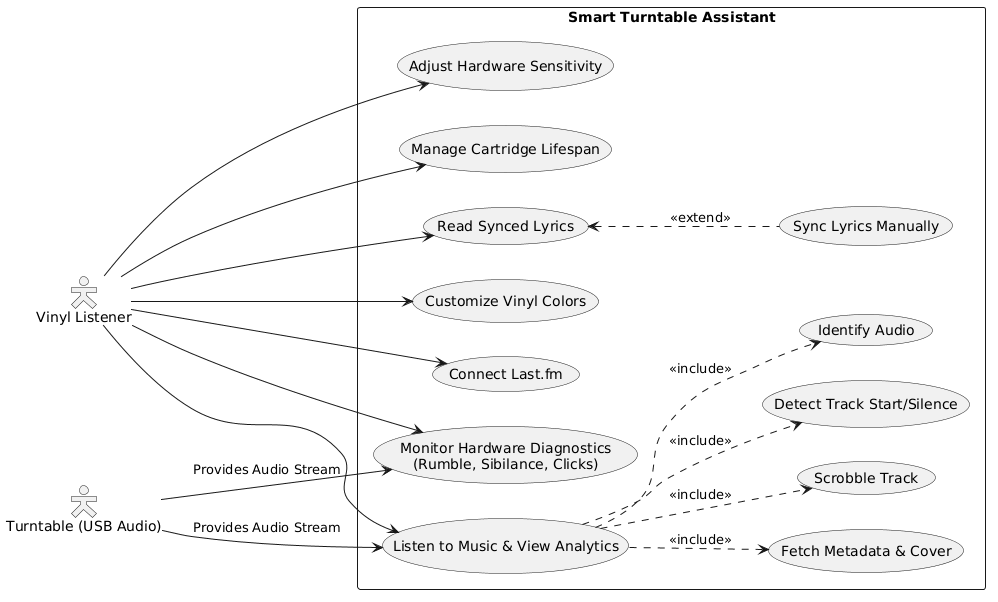
\includegraphics[width=0.8\textwidth]{Images/usecase.png}
    \caption{UML Use Case Diagram illustrating user and system interactions.}
    \label{fig:usecase}
\end{figure}


\chapter{System Design and Architecture}

The transformation of a continuous analog audio signal into a structured, interactive digital experience requires a highly decoupled and concurrent system architecture. This chapter details the structural design of the Smart Turntable Assistant, outlining the client-server communication protocols, the relational database schema, and the complex thread management required to process real-time telemetry alongside asynchronous network requests.

\section{Client-Server Architecture}

The architecture of the application follows a robust client-server model designed to handle both persistent data operations and high-frequency real-time telemetry. The backend is powered by Python and the Flask microframework, acting as the central processing hub that interfaces directly with the audio hardware of the host machine via the Advanced Linux Sound Architecture and PulseAudio subsystems. 

The frontend is a Single Page Application built with the Vue.js framework, serving as the interactive dashboard for the user. Communication between these two distinct environments is bipartite. Standard state mutations, such as user authentication, hardware configuration updates, and manual synchronization adjustments, are handled via stateless Representational State Transfer application programming interfaces. 

Conversely, the continuous stream of audio diagnostics and playback timers necessitates a persistent, low-latency connection. This is achieved utilizing WebSockets through the Socket.IO library. By establishing a full-duplex communication channel, the backend can push mathematical calculations regarding volume, rumble, and sibilance to the frontend multiple times per second, ensuring the user interface remains highly responsive and synchronized with the physical turntable.

\begin{figure}[htbp]
    \centering
    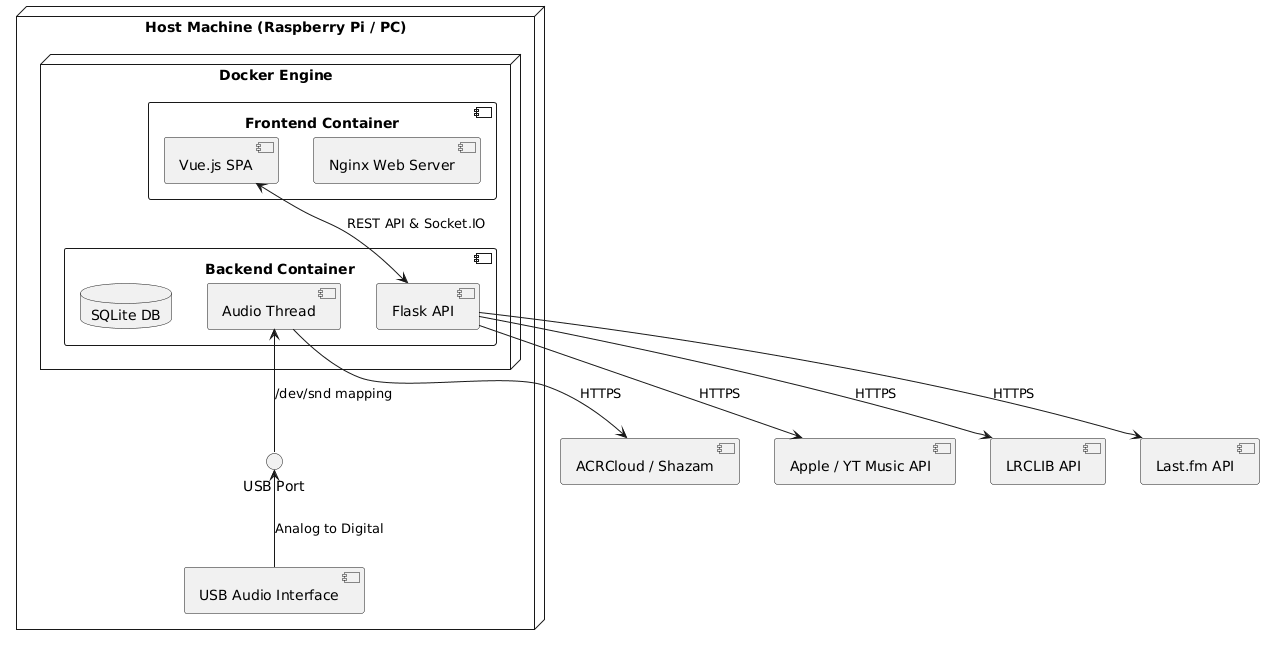
\includegraphics[width=1\textwidth]{Images/deployement.png}
    \caption{Deployment diagram showing Docker containerization and hardware mapping.}
    \label{fig:deployment}
\end{figure}

\section{Database Design}

Persistent data storage is managed by a relational database system, specifically SQLite, integrated through the SQLAlchemy object-relational mapper. The schema is normalized to separate user credentials, hardware metrics, and historical listening habits securely.

At the core of the schema is the User entity, which maintains a one-to-many relationship with all other tables to ensure data isolation in a multi-user environment. The Cartridge table tracks the physical turntable styluses owned by a user, storing their maximum recommended lifespan and the cumulative hours they have been active on the record player. 

The TrackHistory table functions as a digital listening log, recording the identified artist, album, and high-resolution artwork uniform resource locator for every successful audio recognition event. To support the aesthetic and synchronization features of the application, the AlbumColor and TrackOffset tables store user-defined visual preferences and lyric timing calibrations, linking them specifically to the recognized artist and album. This relational structure ensures that when a user logs in, their active stylus limits and previous track modifications are instantly retrieved and applied to the global application state.

\begin{figure}[htbp]
    \centering
    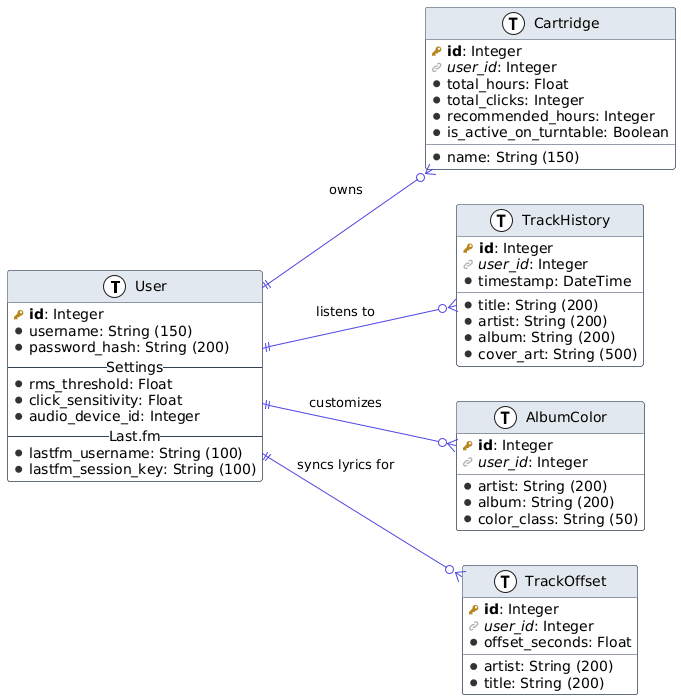
\includegraphics[width=0.85\textwidth]{Images/database.png}
    \caption{Entity-Relationship Diagram of the SQLite database schema.}
    \label{fig:database}
\end{figure}

\section{Concurrency and Thread Management}

Analyzing live audio streams while simultaneously querying external web services presents a significant concurrency challenge. A purely synchronous approach would cause the application to block all diagnostic calculations and freeze the user interface while waiting for a network response from an audio fingerprinting service. To resolve this, the backend employs a multi-threaded architecture orchestrated around a centralized global state object.

The primary audio processing thread runs continuously in the background. It reads distinct blocks of audio from the hardware buffer, calculates root mean square values, detects surface clicks, and updates the active cartridge usage statistics. When this primary thread mathematically determines that a new song has started based on sustained volume thresholds, it spawns an independent, parallel identification thread. 

This secondary thread captures a temporary audio sample and manages the delayed network requests to fingerprinting engines and metadata enrichment application programming interfaces. Because multiple threads interact with the database simultaneously, the SQLite database is configured to use Write-Ahead Logging. This advanced concurrency mode permits the primary thread to safely commit cartridge wear statistics to the disk while the secondary identification thread is actively writing new track history records, completely eliminating database locking errors and ensuring seamless background operation.

\begin{figure}[htbp]
    \centering
    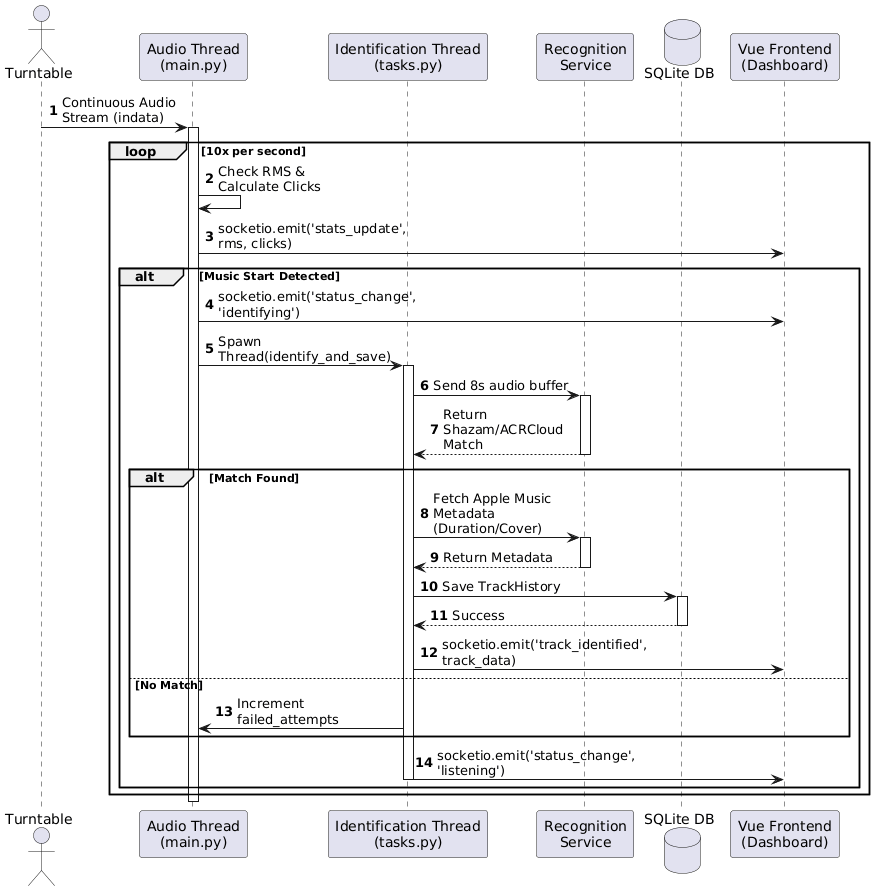
\includegraphics[width=1\textwidth]{Images/sequence.png}
    \caption{UML Sequence Diagram detailing the multithreaded audio identification flow.}
    \label{fig:sequence}
\end{figure}

\chapter{Implementation Details}

Translating the architectural design into a functional application requires precise programming methodologies, robust error handling, and efficient algorithm design. This chapter details the concrete implementation of the Smart Turntable Assistant, exploring the digital signal processing mathematics, the cascading metadata retrieval logic, and the reactive frontend rendering techniques.

\section{Digital Signal Processing}

The core of the application relies on continuously analyzing the analog audio stream provided by the turntable. The Python backend captures audio in discrete mathematical arrays utilizing the sounddevice and NumPy libraries. These data blocks are processed multiple times per second to extract meaningful diagnostic metrics.

To detect when a user drops the needle onto a record, the system calculates the Root Mean Square of the audio chunk, representing the average acoustic energy. If this energy sustains a level above a user-defined threshold for a specific duration, the application registers a playback start event. 

Surface imperfections, such as dust and scratches, manifest as sudden, high-frequency transients known as clicks or pops. The software detects these by calculating the first derivative of the audio signal, which acts as a high-pass filter to isolate rapid changes. By computing the standard deviation of these changes, the algorithm identifies statistical outliers that exceed a specific sensitivity multiplier, successfully counting discrete surface noises.

More advanced diagnostics include mechanical rumble and sibilance tracking. Rumble is calculated by applying a Fast Fourier Transform to the audio array, isolating and summing the acoustic energy present exclusively between ten Hertz and fifty Hertz. Sibilance, which indicates high-frequency tracking distortion, is measured by passing the signal through a Butterworth bandpass filter targeting the five kilohertz to ten kilohertz range. The energy of this isolated band is compared as a ratio against the overall signal energy, yielding a percentage that dynamically drives the harshness meter on the frontend interface.

\section{The Waterfall Metadata Strategy}

Relying on a single external service for music identification and metadata often results in incomplete information, especially for underground or niche musical genres. To solve this, the application employs a cascading waterfall strategy that queries multiple application programming interfaces in a strict priority sequence.

The process begins by recording an eight-second audio sample and submitting it asynchronously to audio fingerprinting engines. If a match is found, the system extracts the unique Apple Music identifier embedded within the payload. This specific identifier allows the backend to query the iTunes web service directly, guaranteeing the retrieval of the exact track duration in milliseconds, the official album name, and a high-resolution square album cover.

If the primary fingerprinting service fails to provide an exact identifier, the system falls back to a text-based search utilizing the ytmusicapi library. This library scrapes the official YouTube Music catalog. To ensure the frontend receives high-quality artwork instead of low-resolution video thumbnails, the software manipulates the dynamically generated image uniform resource locator by replacing the default dimension parameters with strict high-resolution requests, yielding perfectly sharp imagery for the user interface.

\section{Backend State Management and Data Streaming}

Managing the flow of data between parallel background threads and connected web clients requires a centralized source of truth. The backend implements a global state object that holds the current track metadata, live diagnostic values, and playback timers. 

Because the audio processing thread evaluates data ten times per second, writing cartridge usage statistics directly to the SQLite database at that frequency would cause severe input and output bottlenecks and degrade the storage medium. Instead, the system accumulates playback seconds and click counts in temporary memory variables. A throttling mechanism ensures that these accumulated values are only committed to the physical database once every ten seconds. Concurrently, the live values are broadcast over the Socket.IO connection to all connected clients, ensuring the frontend displays fluid, real-time animations without overwhelming the server hardware.

\section{Frontend Interface and Reactive Architecture}

The user interface is engineered as a Single Page Application using the Vue.js framework, designed to decouple the visual presentation from the backend logic.

\subsection{Client State and Routing}

Global client state, including user authentication and session tokens, is managed by the Pinia state management library. This ensures that when a user refreshes the page, their session persists by reading credentials directly from the local storage of the browser. The Vue Router intercepts all navigation attempts, verifying the authentication state before granting access to the primary dashboard or the user profile configuration pages.

\subsection{Dynamic Styling and Theming}

The graphical interface is built to be entirely responsive, utilizing modern cascading style sheet features such as container queries and fluid typography clamp functions. This guarantees that the visual record player and text elements scale proportionately whether viewed on a mobile device or a high-resolution desktop monitor. 

The aesthetic presentation is governed by dynamic data attributes applied to the root document element. By toggling these attributes, the application instantly swaps extensive sets of cascading style sheet variables. This mechanism allows the user to transition the interface from a modern, rounded aesthetic with smooth gradients into a boxy, highly contrasted retro interface inspired by legacy operating systems, completely transforming the user experience without requiring a page reload.

\subsection{Synchronized Lyrics Rendering}

When a track is identified, the backend queries an open-source lyric database to retrieve text formatted with precise synchronization timestamps. The frontend parses this text string into an array of mathematical objects. A reactive computed property continuously compares these timestamps against the live track timer broadcast by the backend. When the timer surpasses a lyric timestamp, the active index updates, and the application triggers a smooth scroll event. The software utilizes the next tick rendering cycle of the Vue framework to ensure the document object model has fully updated before attempting to scroll the active line directly into the center of the viewport.

\section{Third-Party Integrations}

To bridge the gap between analog playback and digital tracking, the software integrates heavily with the Last.fm social music platform. The application implements a web authentication flow where the user authorizes the software, returning a temporary token. 

Because standard Python libraries frequently fail to parse this token correctly due to strict formatting rules, the backend bypasses third-party wrappers for the authentication step. Instead, it manually constructs an MD5 hashed security signature containing the developer secrets and the token, sending a direct network request to the Last.fm servers to retrieve a permanent session key. During playback, a background thread monitors the elapsed track time. Once the track reaches exactly fifty percent completion or four minutes of continuous playback, a secondary background process securely transmits the artist and title data to the Last.fm servers, successfully cataloging the analog listening session into the digital profile of the user.

\chapter{Testing and Evaluation}

To ensure the Smart Turntable Assistant operates reliably under real-world conditions, a rigorous testing and optimization phase was conducted. This chapter details the integration testing of the hardware and software components, as well as the specific performance optimizations required to run continuous audio analysis on constrained computing devices.

\section{Manual and Integration Testing}

The system was evaluated using a variety of physical vinyl records encompassing different genres, pressing qualities, and surface conditions. The audio input stream was heavily scrutinized to verify the accuracy of the digital signal processing algorithms. Records with known physical damage were played to confirm that the click detection logic accurately incremented the error counter without registering false positives from aggressive drum transients. Similarly, the sibilance and rumble meters were monitored against records with known tracking distortion and turntable setups with intentional motor vibration, proving the mathematical validity of the frequency analysis. 

The integration between the frontend interface and the backend server was tested by manipulating the graphical user interface during active playback. Triggering manual track detection, adjusting the synchronized lyric timeline by fractional seconds, and rapidly switching visual themes all performed flawlessly without interrupting the continuous WebSocket telemetry broadcast. The cascading metadata retrieval system successfully identified obscure tracks by falling back to secondary music databases when the primary audio fingerprinting engine failed to provide complete information.

\section{Performance Optimization}

Running continuous audio analysis algorithms alongside a web server on constrained hardware requires strict resource management. Initial testing revealed that writing cartridge health statistics to the database multiple times per second caused severe input and output bottlenecks, ultimately crashing the application with database locked errors. 

To resolve this, the database engine was reconfigured to utilize Write-Ahead Logging, an advanced journaling mode that allows simultaneous read and write operations across different background threads. Furthermore, a memory buffering system was implemented within the main execution loop. Instead of interacting with the database continuously, the primary audio thread accumulates elapsed playback seconds and click events in temporary variables. The system commits the combined totals to the persistent storage drive only once every ten seconds. This optimization significantly reduced processor load and minimized physical write cycles, ensuring the longevity of the solid-state storage medium while maintaining a highly responsive user experience.

\chapter{Conclusion and Future Work}

The final chapter summarizes the outcomes of the development process, evaluating the success of the implemented features against the initial objectives, and explores potential avenues for future research and software expansion.

\section{Evaluation of Achieved Results}

The Smart Turntable Assistant successfully achieves its primary objective of modernizing the analog vinyl listening experience. By passively monitoring the raw electrical audio signal, the system bridges the gap between physical media and the digital ecosystem. The application accurately identifies playing tracks, enriches the listening session with high-resolution artwork and synchronized lyrics, and seamlessly logs playback history to external social music platforms. 

Furthermore, the inclusion of audiophile-grade diagnostic tools provides users with unprecedented, real-time visual feedback regarding the physical health of their stylus and their records. The highly modular, decoupled architecture ensures that the underlying Python backend and the reactive web interface operate efficiently, culminating in a professional and robust software solution that honors the traditional vinyl medium while providing modern digital conveniences.

\section{Future Development Opportunities}

While the current implementation fulfills all initial requirements, several avenues exist for future enhancement. The most significant potential upgrade involves developing a proprietary audio fingerprinting algorithm to run entirely locally on the host hardware. This feature would remove all dependencies on third-party recognition engines and eliminate the need for an active internet connection during the identification phase. 

Additionally, the diagnostic suite could be expanded to include an automated turntable calibration mode. By analyzing standardized analog test tones, the software could help users perfectly align their cartridge azimuth and anti-skate mechanisms mathematically. Finally, integrating the audio capture stream with open-source multi-room casting protocols would allow users to wirelessly broadcast their analog records to smart speakers throughout their home, further expanding the utility of the system.

\end{document}